\section{Modèle Physique et simulation}


\subsection{Fonctionnement du modèle d'Ising}

Comme expliqué en introduction, le modèle d'Ising consiste en un assemblage d'éléments possédant un moment magnétique positif ou négatif.

Dans le cas physique qui nous intéresse le système représente un système thermodynamique : un solide cubique.
Les moments magnétiques sont ceux des électrons de valence qui composent le solide.




On peut mettre des mots en \emph{italique}, 
en \textsc{petites Majuscules} ou 
en \texttt{largeur fixe (machine à écrire)}.

Voici un deuxième paragraphe avec une formule mathématique simple : $e = mc^2$.


\subsubsection{Observations attendues}

\foreignlanguage{english}{Do you speak French? Does anybody here speak french?}


\subsection{Simulation informatique}

\begin{itemize}
\item Liste classique ;
\item un élément ;
\item et un autre élément.
\end{itemize}
\vspace{\parskip} % espace entre paragraphes

\begin{enumerate}
\item Une liste numéroté
\item deux
\item trois
\end{enumerate}
\vspace{\parskip}

\begin{description}
\item[Description] C'est bien pour des définitions.
\item[Deux] Ou pour faire un liste spéciale.
\end{description}
\vspace{\parskip}

\subsubsection{La méthode Métropolis}

\subsubsection{Structure et fonctionnement du programme}

\begin{figure}[!ht]
    \center
    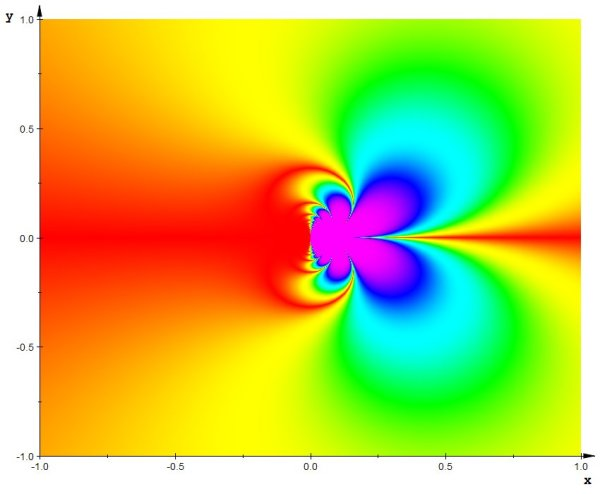
\includegraphics[]{./images/exemple.jpg}
    \caption{taille original}
    \label{Diagramme UML du programme}
\end{figure}
